
\section{ICE}

\subsection{Introduction}

\subsection{Theory - Algorithm Description}

\subsection{Uintah Specification}

\subsubsection{Basic Inputs}
\subsubsection{Physical Constants}
\subsubsection{Material Properties}
\subsubsection{Equation of State}
\subsubsection{Exchange Properties}
\subsubsection{BoundaryConditions}
\subsubsection{Solvers}
%______________________________________________________________________
\subsection{Examples}
\section*{\center Shock Tube}
\subsection*{\underline{Problem Description}}
The shock tube problem is a standard 1D compressible flow problem that
has been used by many as a validation test case \cite{laney, sod, toro}.
At time $t=0$ the computational domain is divided into two separate regions of
space by a diaphram, with each region at a different density and pressure.
The separated regions are at rest with a uniform temperature $=300K$.
The initial pressure ratio is $\frac{P_R}{P_L}  = 10$ and density ratio
is $\frac{\rho_R}{\rho_L} = 0.1$  The diaphram is instantly removed and a
traveling shockwave, discontinutity and expansion fan form.  The expansion
fan moves towards the left while the shockwave and contact discontinutity
move to the right.  This problem tests the algorithm's ability to capture
steep gradients and solve Eulers equations.

 
\subsection*{\underline{Simulation Specifics}}
\begin{description} 
\small
\item [Component used:] \hfill ICE
\item [Input file name:] \hfill inputs/ICE/rieman\_sm.ups
\item [Command used to run input file:]\hfill sus inputs/UintahRelease/ICE/shockTube.ups
\item [Postprocessing command:]\hfill \\
inputs/UintahRelease/ICE/plot\_shockTube\_1L shockTube.uda y \\
This will generate a postscript file shockTube.ps

\item [Simulation Domain:]\hfill    1 x .001 x .001 m
\item [Cell Spacing:]\hfill \\ 
1 x 1 x 1 mm (Level 0)

\item [Example Runtimes:] \hfill \\
 1 minutes   (1 processor, 2.66 GHz Xeon)

\item [Physical time simulated:] \hfill 0.005 sec.

\end{description}

\section*{\underline{Results}}
Figure \ref{results.ST} shows a comparison of the exact versus simulated
results at time $t = 5msec$.

\begin{figure}
  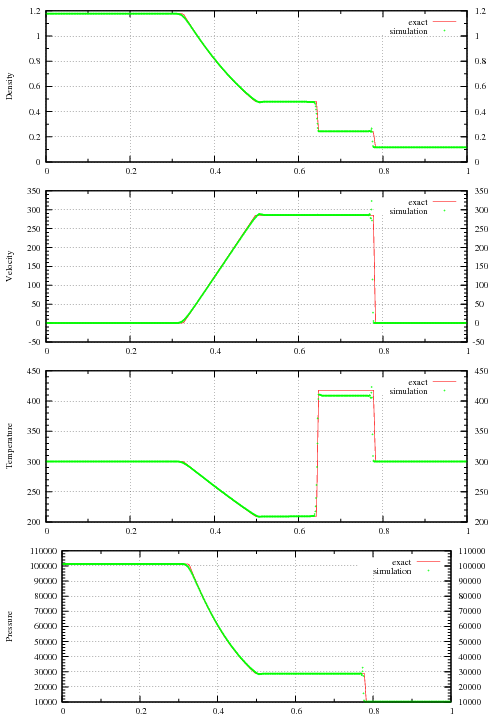
\includegraphics[scale=.85]{shockTube.png}
  \caption{Shock tube results at time $t = 5msec$}
  \label{results.ST}
  \end{figure}
\newpage

%__________________________________SHOCKTUBE AMR

\section*{\center Shock Tube with AMR}
 
\subsection*{\underline{Simulation Specifics}}
\begin{description} 
\small
\item [Component used:] \hfill ICE
\item [Input file name:] \hfill shocktube\_AMR.ups
\item [Command used to run input file:]\hfill sus inputs/UintahRelease/ICE/shocktube\_AMR.ups
\item [Postprocessing command:]\hfill \\
inputs/UintahRelease/ICE/plot\_shockTube\_AMR shockTube\_AMR.uda y
This will generate a postscript file shockTube\_AMR.ps

\item [Simulation Domain:]\hfill    1 x .001 x .001 m
\item [Cell Spacing:]\hfill 
10 x 1 x 1 mm (Level 0)\\
2.5 x 1 x1 mm (Level 1)\\
0.625 x1 x1 mm (Level 2)

\item [Example Runtimes:] \hfill \\
 2ish minutes   (1 processor, 2.66 GHz Xeon)

\item [Physical time simulated:] \hfill 0.005 sec.

\end{description}

\section*{\underline{Results}}
Figure \ref{results.ST.AMR} shows a comparison of the exact versus simulated results at time $t = 5msec$.
\begin{figure}
  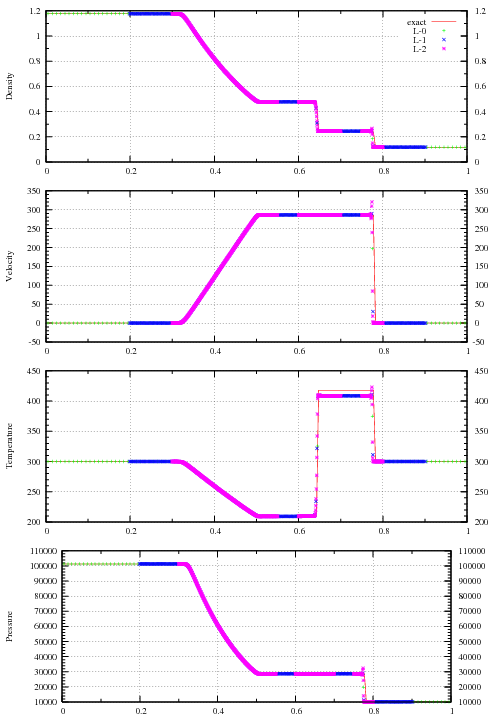
\includegraphics[scale=.85]{shockTube_AMR.png}
  \caption{Shock tube results at time $t = 5msec$}
  \label{results.ST.AMR}
  \end{figure}
\newpage

%__________________________________riemann2D

\section*{\center 2D Riamann Problem with AMR}
\subsection*{\underline{Problem Description}}
In two-dimensional Riemann problems there 15 different solutions that combine rarefaction waves, shock waves and a slip line or contact discontinuities \cite{ref:schulz_collins_glaz, ref:Liska_Wendroff}.  Here we simulate 4 slip lines that form a symmetrical single vortex turning counter clockwise. At time $t=0$ the computational domain is divided into four quadrants by the lines $x = 1/2, y=1/2$  The initial condition for $V=(p, \rho, u, v)$ in the four quadrants are $V_{ll}=(1, 1, -0.75, 0.5), V_{lr}=(1, 3, -0.75,-0.5), V_{ul}=(1,2,0.75,0.5), V_{ur}=(1,1,0.75,-0.5)$ where, $p$ is pressure, $\rho$ is the density of the polytropic gas, $u$ and $v$ are the $x$ and $y$ component of velocity.
\subsection*{\underline{Simulation Specifics}}
\begin{description} 
\small
\item [Component used:] \hfill ICE
\item [Input file name:] \hfill riemann2D\_AMR.ups
\item [Command used to run input file:]\hfill mpirun -np 5 sus inputs/UintahRelease/ICE/riemann2D\_AMR.ups
\item [VisIT session file:]\hfill inputs/UintahRelease/ICE/riemann2D.session
\item [Simulation Domain:]\hfill    0.96 x 0.96m x 0.1 m
\item [Cell Spacing:]\hfill \\ 
40  x 40  x 1 mm (Level 0)\\
10  x 10  x 1 mm (Level 1)\\
2.5 x 2.5 x 1 mm (Level 2)

\item [Example Runtimes:] \hfill \\
 5ish minutes   (5 processors, 2.66 GHz Xeon)
\item [Physical time simulated:] \hfill 0.3 sec.
\end{description}

\section*{\underline{Results}}
Figure \ref{fig:riemann2D} shows a flood and line contour plot(s) of the density of the gas at 0.03sec.
\begin{figure}
  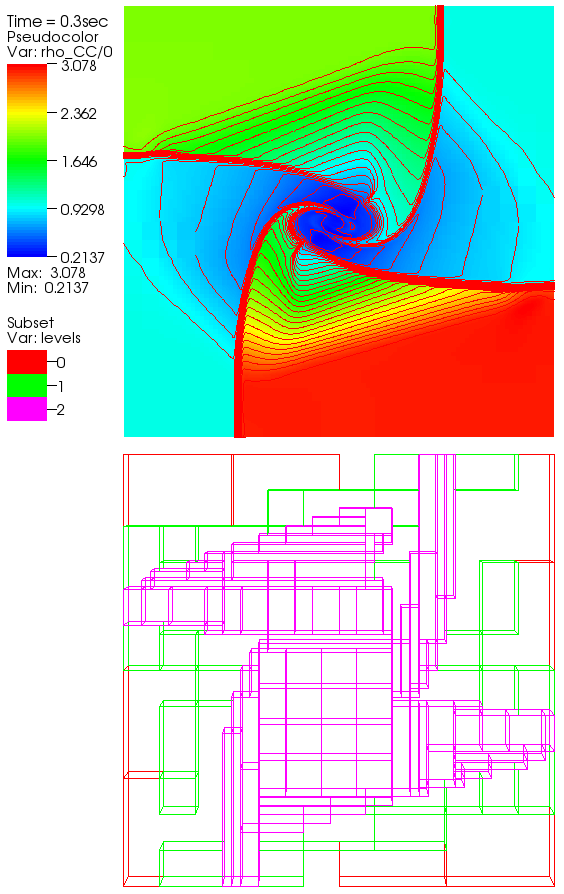
\includegraphics[scale=.6]{riemann2D.png}
  \caption{Contour plot of density for the 2D Riemann problem at time $t = 0.3sec$.  Bottom plot shows the outline of the patches on the 3 levels.}
  \label{fig:riemann2D}
  \end{figure}
\newpage

%__________________________________Single level blast wave

\section*{\center BlastWave 2D}
\subsection*{\underline{Problem Description}}
The Sedov-Taylor blastwave problem is a standard compressible flow problem
that has been used by many as a validation test case.  At time $t=0$ there
is a small region of gas at the center of the domain at a relatively high
temperature and pressure.  The expansion of high pressure gas forms a
spherical blast wave that expands into surrounding atmosphere.
\subsection*{\underline{Simulation Specifics}}
\begin{description} 
\item [Component used:] \hfill ICE
\item [Input file name:] \hfill blastWave.ups
\item [Command used to run input file:]\hfill sus blastWave.ups
\item [Visualization net file:]\hfill blastWave\_1L.srn\\


\item [Simulation Domain:]\hfill    1 x 1 x .05 m
\item [Cell Spacing:]\hfill \\ 
5 x 5 x 50 mm (Level 0)


\item [Example Runtimes:] \hfill \\
 9ish minutes   (1 processor, 2.66 GHz Xeon)

\item [Physical time simulated:] \hfill 0.9e-3sec.

\end{description}

\section*{\underline{Results}}
Figure \ref{results.BW} shows a comparison of the exact versus simulated
results at time $t = 5msec$.

\begin{figure}
  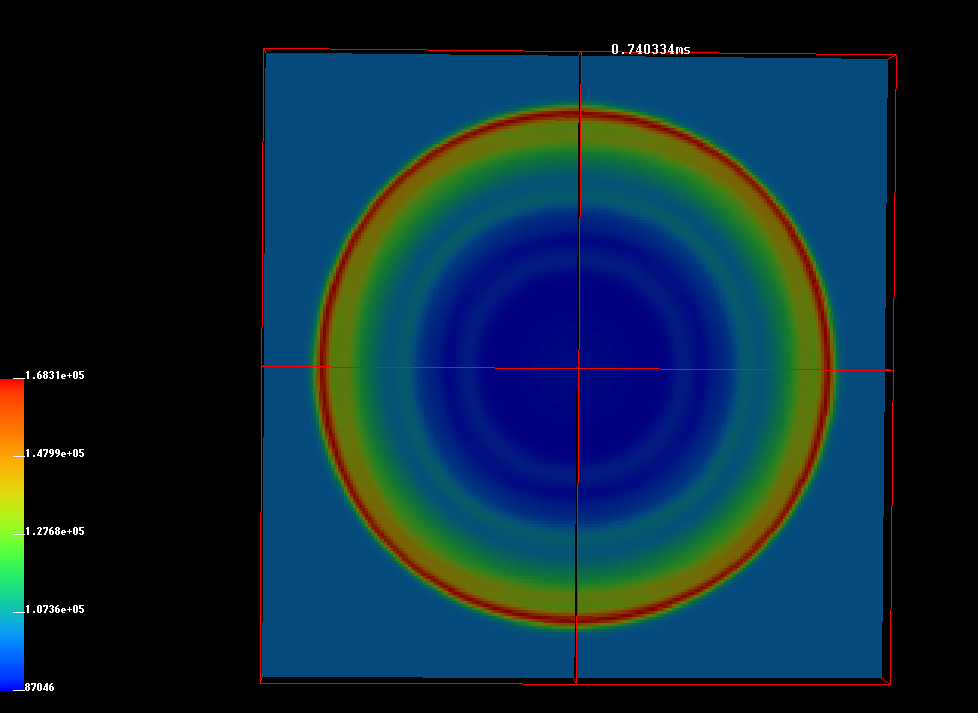
\includegraphics[scale=.5]{blastWave.png}
  \caption{Pressure field at time $t = 0.74msec$}
  \label{results.BW}
  \end{figure}
\newpage

%__________________________________AMR blast wave

\section*{\center BlastWave AMR}
\subsection*{\underline{Simulation Specifics}}
\begin{description} 
\item [Component used:] \hfill ICE
\item [Input file name:] \hfill blastWave.ups
\item [Command used to run input file:]\hfill sus blastWave\_AMR.ups
\item [Visualization net file:]\hfill blastWave\_1L.srn\\


\item [Simulation Domain:]\hfill    1 x 1 x .05 m
\item [Cell Spacing:]\hfill \\ 
20 x 20 x 50 mm (Level 0) 
5 x 5 x 50 mm (Level 1)


\item [Example Runtimes:] \hfill \\
 9ish minutes   (1 processor, 2.66 GHz Xeon)

\item [Physical time simulated:] \hfill 0.9e-3sec.

\end{description}

\section*{\underline{Results}}
Figure \ref{results.BW.AMR} shows the pressure field and an outline of the
individual patches on levels 0 \& 1.  This simulation shows the adaptive
mesh capabilities of ICE and the UCF.
\begin{figure}
  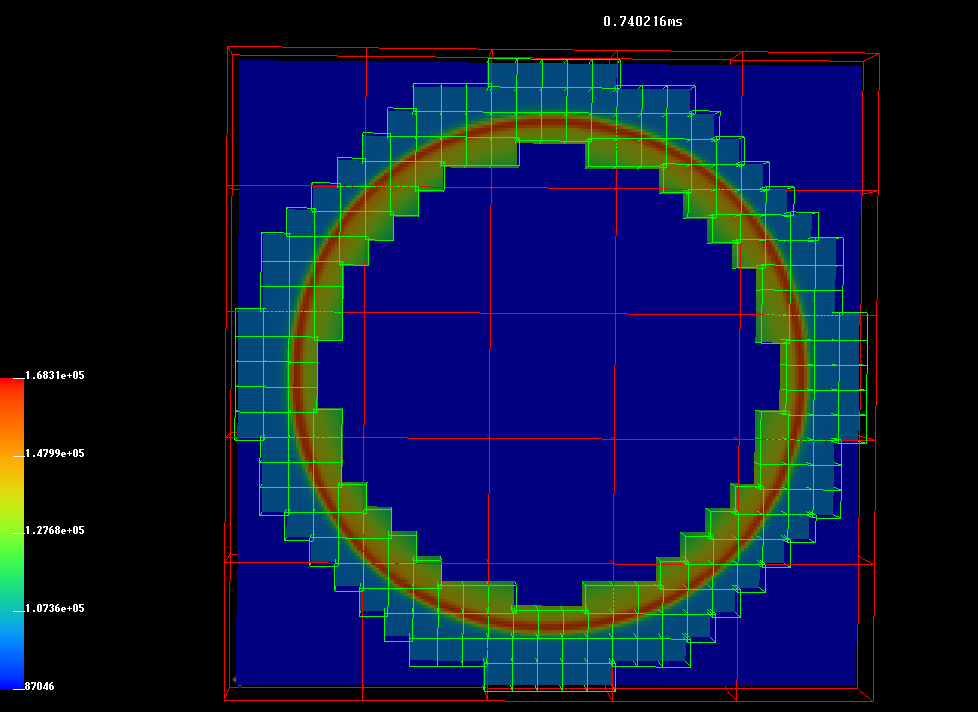
\includegraphics[scale=.5]{blastWave_AMR.png}
  \caption{Pressure field at time $t = 0.74msec$.  The individual patches on levels 0 \& 1 are shown.}
  \label{results.BW.AMR}
  \end{figure}
Good agreement between the single level results (Fig. \ref{results.BW}) and the AMR results (Fig.
\ref{results.BW.AMR}) is shown.
\newpage

%__________________________________CH4 fire

\section*{\center Methane Flame}
\subsection*{\underline{Problem Description}}
At $t=0$ Methane gas begin flowing from a $1m$ hole in the floor of the
computational domain at a velocity of $1m/s$.  The methane mixes with the
surrounding air, ignites and forms a puffing fire.  The main assumptions in
this simulation are a) that the chemical reactions are taking place infinitely
fast (equilibrium chemistry model) and b) that there is no radiative heat
loss from the product gases.
\subsection*{\underline{Simulation Specifics}}
\begin{description} 
\item [Component used:] \hfill ICE
\item [Input file name:] \hfill CH4\_fire.ups
\item [Command used to run input file:]\hfill sus CH4\_fire.ups \\
Note you must have a link to the {\tt inputs} directory in the save directory as sus.  A table needed
by the combustion model is inside the {\tt inputs} directory.
\item [SCIRun visualization net file:]\hfill 3DFire\_Vol.srn \\


\item [Simulation Domain:]\hfill    5 x 5 x 5 m
\item [Cell Spacing:]\hfill \\ 
3.3 x 3.3 x 3.3 cm (Level 0)


\item [Example Runtimes:] \hfill \\
 8 hours   (64 processor, 2.66 GHz Xeon)

\item [Physical time simulated:] \hfill 3.4sec.

\end{description}

\section*{\underline{Results}}
Figure \ref{results.CH4} shows a 3D view of the initial puff just before it leaves the computational
doman.  
\begin{figure}
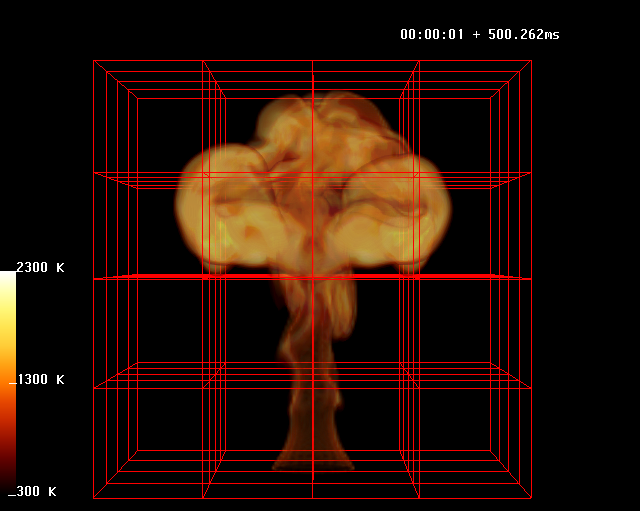
\includegraphics[scale=.66]{3DFire.png}
\caption{Temperature field at time $t = 1.5 sec$}
\label{results.CH4}
\end{figure}
\newpage


\subsection{References}
\bibliography{ice}


